\chapter{Long Short-Term Memory (LSTM) \cite{dnn-1}}


\begin{figure}[H]
    \centering
    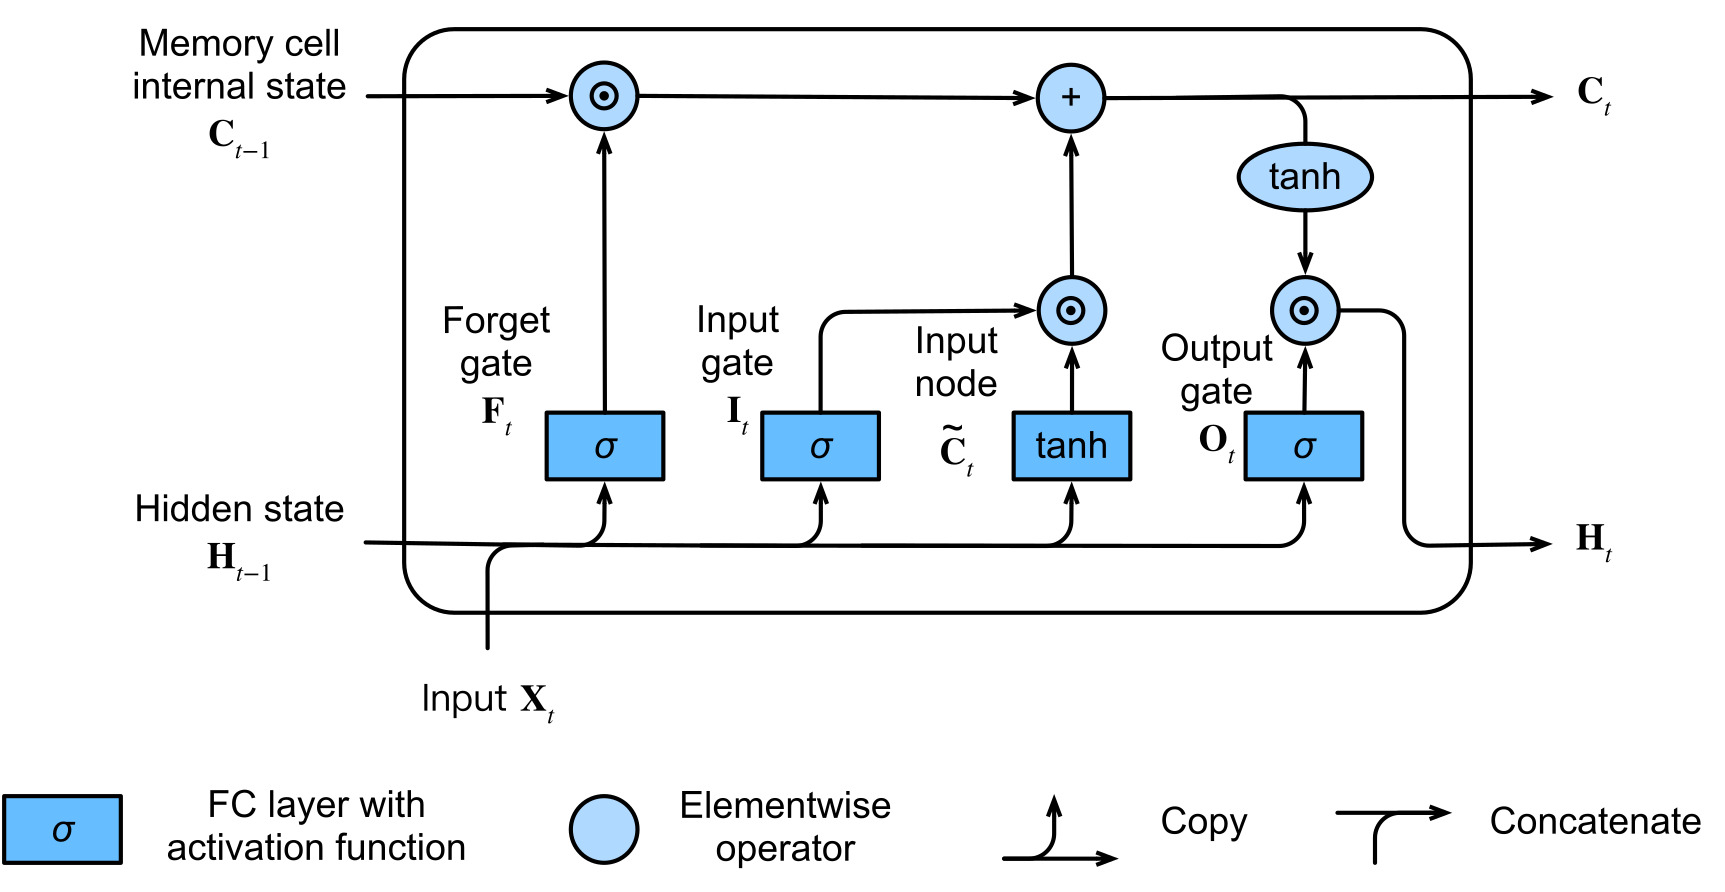
\includegraphics[width=\linewidth, height=5cm, keepaspectratio]{Pictures/lstm/lstm-final.jpg}
\end{figure}

\begin{customTableWrapper}{1.5}
\begin{longtable}{l l p{8cm}}
    \hline
    \customTableHeaderColor
    \multicolumn{3}{c}{Inputs} \\ \hline

    $n$ & $\in \mathbb{R}$ & batch size \\
    
    $d$ & $\in \mathbb{R}$ & number of inputs \\
    
    $t$ & $\in \mathbb{R}$ & time step \\
    
    $\mathbf{X}_t$ & $\in \mathbb{R}^{n \times d}$ & input \\

    \hline
    \customTableHeaderColor
    \multicolumn{3}{c}{Hidden State} \\ \hline

    $h$ & $\in \mathbb{R}$ & number of hidden units \\
    $\mathbf{H}_{t-1}$ & $\in \mathbb{R}^{n \times h}$ & hidden state of the previous time step \\


    \hline
    \customTableHeaderColor
    \multicolumn{3}{c}{Input Gate} \\ \hline

    $\mathbf{W}_{\textrm{xi}}$ & $\in \mathbb{R}^{d \times h}$ & weight parameter \\
    $\mathbf{W}_{\textrm{hi}}$ & $\in \mathbb{R}^{h \times h}$ & weight parameter \\
    $\mathbf{b}_\textrm{i}$ & $\in \mathbb{R}^{1 \times h}$ & bias parameter \\
    $\mathbf{I}_t$ & $\in \mathbb{R}^{n \times h}$ & input gate \\

    \hline
    \customTableHeaderColor
    \multicolumn{3}{c}{Forget Gate} \\ \hline

    $\mathbf{W}_{\textrm{xf}}$ & $\in \mathbb{R}^{d \times h}$ & weight parameter \\
    $\mathbf{W}_{\textrm{hf}}$  & $\in \mathbb{R}^{h \times h}$ & weight parameter \\
    $\mathbf{b}_\textrm{f}$ & $\in \mathbb{R}^{1 \times h}$ & bias parameter \\
    $\mathbf{F}_t$ & $\in \mathbb{R}^{n \times h}$ & forget gate \\

    \hline
    \customTableHeaderColor
    \multicolumn{3}{c}{Output Gate} \\ \hline

    $\mathbf{W}_{\textrm{xo}}$ & $\in \mathbb{R}^{d \times h}$ & weight parameter \\
    $\mathbf{W}_{\textrm{ho}}$ & $\in \mathbb{R}^{h \times h}$ & weight parameter \\
    $\mathbf{b}_\textrm{o}$ & $\in \mathbb{R}^{1 \times h}$ & bias parameter \\
    $\mathbf{O}_t$ & $\in \mathbb{R}^{n \times h}$ & output gate \\



\end{longtable}
\end{customTableWrapper}



\begin{enumerate}
    \item LSTMs resemble standard recurrent neural networks but here each ordinary recurrent node is replaced by a \textbf{memory cell}.

    \item The LSTM model introduces an intermediate type of storage via the memory cell. 
    
    \item Each memory cell contains an \textbf{internal state}, i.e., a node with a self-connected recurrent edge of fixed weight 1, ensuring that the gradient can pass across many time steps without vanishing or exploding.
    
    \item A memory cell is a composite unit, built from simpler nodes in a specific connectivity pattern, with the novel inclusion of multiplicative nodes.

    \item Simple recurrent neural networks have \textbf{long-term memory} in the form of weights.\\
    The weights change slowly during training, encoding general knowledge about the data. \\
    They also have short-term memory in the form of ephemeral activations, which pass from each node to successive nodes. 

    
\end{enumerate}




\section{Gated Memory Cell \cite{dnn-1}} \label{lstm: Gated Memory Cell}

\begin{enumerate}
    \item Each memory cell is equipped with an internal state and a number of multiplicative gates that determine whether 
    \begin{enumerate}
        \item a given input should impact the internal state (the \textbf{input gate})
        \item the internal state should be flushed to $0$ (the \textbf{forget gate})
        \item the internal state of a given neuron should be allowed to impact the cell’s output (the \textbf{output gate})
    \end{enumerate}

    \item The key distinction between vanilla RNNs and LSTMs is that the latter support gating of the hidden state. \\
    This means that we have dedicated mechanisms for when a hidden state should be \textbf{updated} and also for when it should be \textbf{reset}.

    \item For instance, if the first token is of great importance we will learn \textbf{not to update} the hidden state after the first observation. \\
    Likewise, we will learn to \textbf{skip} irrelevant temporary observations. \\
    Last, we will learn to \textbf{reset} the latent state whenever needed.

\end{enumerate}


\section{Components of LSTM \cite{dnn-1}}

\begin{enumerate}[itemsep=0.15cm]
    \item The data feeding into the LSTM gates are the input at the current time step and the hidden state of the previous time step

    \item \textbf{Input node}
    \begin{enumerate}
        \item 

    \end{enumerate}

    \item \textbf{Input Gate}
    \begin{enumerate}
        \item $\mathbf{I}_t = \sigma(\mathbf{X}_t \mathbf{W}_{\textrm{xi}} + \mathbf{H}_{t-1} \mathbf{W}_{\textrm{hi}} + \mathbf{b}_\textrm{i})$

        \item As a result of the sigmoid activation, values of the gate is in the range of $(0,1)$

        \item Intuitively, the input gate determines how much of the input node’s value should be added to the current memory cell internal state.

        \item Note that broadcasting is triggered during the summation. (SEE \fullref{Broadcasting in matrices})
    \end{enumerate}

    \item \textbf{Forget Gate}
    \begin{enumerate}
        \item $\mathbf{F}_t = \sigma(\mathbf{X}_t \mathbf{W}_{\textrm{xf}} + \mathbf{H}_{t-1} \mathbf{W}_{\textrm{hf}} + \mathbf{b}_\textrm{f})$

        \item As a result of the sigmoid activation, values of the gate is in the range of $(0,1)$

        \item The forget gate determines whether to keep the current value of the memory or flush it.

        \item Note that broadcasting is triggered during the summation. (SEE \fullref{Broadcasting in matrices})
    \end{enumerate}

    \item \textbf{Output Gate}
    \begin{enumerate}
        \item $\mathbf{O}_t = \sigma(\mathbf{X}_t \mathbf{W}_{\textrm{xo}} + \mathbf{H}_{t-1} \mathbf{W}_{\textrm{ho}} + \mathbf{b}_\textrm{o})$
    
        \item As a result of the sigmoid activation, values of the gate is in the range of $(0,1)$

        \item the output gate determines whether the memory cell should influence the output at the current time step.

        \item Note that broadcasting is triggered during the summation. (SEE \fullref{Broadcasting in matrices})
    \end{enumerate}


\end{enumerate}













